%%%%%%%%%%%%%%%%%%%%%%%%%%%%%%%%%%%%%%%%%%%%
% Chapitre 2
%%%%%%%%%%%%%%%%%%%%%%%%%%%%%%%%%%%%%%%%%%%%


\chapter{La diffusion pour la médecine}
\label{Chapter2}

Nous avons vu dans le chapitre précédent (\chapref{Chapter1}) que l'\itd permet de visualiser \textit{in vivo}
la diffusion des molécules d'eau dans les tissus cérébraux.
De plus, nous avons introduit les différentes notions mathématiques associées au tenseur de diffusion,
avec notamment la présentation de la géométrie du tenseur sous forme d'ellipsoïde.

Ce deuxième chapitre sert à faire le lien entre ces notions et celles de l'anatomie cérébrale 
ainsi que des pathologies dégénératives du système nerveux centrale chez l'homme.

Il s'agit de comprendre, dans un premier temps, pourquoi nous utilisons l'ITD
pour étudier le processus des pathologies dégénératives.
Puis, dans un deuxième temps, de voir quelles sont les limites d'une telle modalité d'imagerie pour ces cas d'étude.
Enfin, il semble important d'expliquer en quoi l'étude de ces pathologies est cruciale dans la recherche clinique.
Ce chapitre se concentrera sur le système nerveux central chez l'homme et sur des pathologies de type démence.

\begin{figure*}[h]
    \centering
    
\includegraphics[width=0.5\textwidth]{Images/lechat.jpg}
    \caption{\label{fig:lechat} Illustration du dessinateur Philippe Geluck.}
\end{figure*}

%----------------------------------------------------------------------------------------

\section{Anatomie du système nerveux centrale}
La désignation \og système nerveux central chez l'homme \fg englobe trois structures anatomiques différentes : 
le cerveau, le cervelet et la moelle épinière.
Seule la partie supérieure de cette dernière (bien qu'étant une structure à part entière) 
qui fait la jonction entre elle et la partie inférieure du cerveau sera exploitée.

Le cerveau est une structure anatomique qui baigne dans du liquide céphalorachidien (LCR) 
et qui est composée de deux types de substances : la substance blanche et la substance grise.
En tout, ce sont trois tissus ayant des propriétés de diffusion de l'eau différentes : 
le liquide céphalorachidien (LCR) et la substance grise présentent une diffusion isotropique 
et la substance blanche ayant une diffusion anisotropique.
La \figref{fig:trois_substances} représente une coupe axiale d'une image cérébrale avec des indications 
sur les différents tissus qui composent le cerveau.

\begin{figure}[ht]
    \centering
    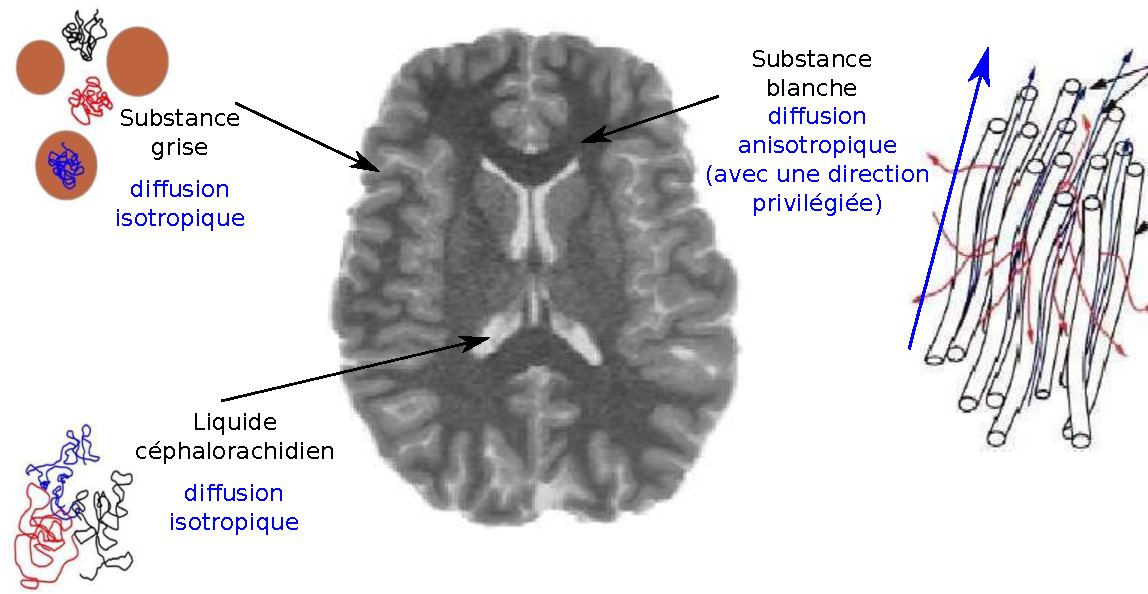
\includegraphics[width=1\textwidth]{Images/tissus_fr.pdf}
    \caption{\label{fig:trois_substances}Illustration (coupe axiale) des trois substances principales 
    composant le cerveau humain avec leurs propriétés propres de diffusion de l'eau : 
    le liquide céphalorachidien ($=$ diffusion isotropique), la substance grise ($=$ diffusion isotropique) 
    et la substance blanche ($=$ diffusion anisotropique). }
\end{figure}

Le liquide céphalorachidien est un fluide et, par conséquence, aucune contrainte n'est exercée sur les molécules d'eau 
qui se déplacent librement : elles ont un mouvement Brownien.
Cela se traduit par une valeur de DM élevée ($\varnothing$ structure)
et une valeur de FA proche de zéro ($\varnothing$ restriction spatiale).

La substance grise contient les corps cellulaires des neurones. 
Ils ne guident pas particulièrement les molécules d'eau suivant une certaine direction (FA faible).
Mais la structure des tissus a pour effet de bloquer la diffusion isotropique des molécules entre les corps cellulaires.
Par conséquent, les valeurs de diffusion moyenne sont faibles.

En ce qui concerne la substance blanche, elle est composée d'axones gainés de myéline qui relient les neurones entre eux.
Cette gaine a un rôle déterminant car elle protège l'axone et permet de mieux transmettre l'influx nerveux entre les neurones.
L'analogie entre cette gaine de myéline et une gaine d'un câble électrique est souvent utilisée pour imager ses propriétés conductrices.
Dans la substance blanche, les axones (ou fibres) se regroupent entre eux pour former des faisceaux reliant diverses régions anatomiques du cerveau.
Un exemple illustratif est celui du corps calleux où les fibres de la substance blanche traversent le cerveau 
pour connecter les hémisphères gauche et droit (\figref{fig:tracto_corps_calleux}).
Dans un faisceau, les molécules d'eau sont entourées d'axones ce qui impose une restriction de leurs déplacements suivant deux directions
et qui priviligie la direction correspondante à celle des axones.
De ce fait, les valeurs de FA dans ce tissu sont élevées.

\begin{figure}[ht]
    \centering
    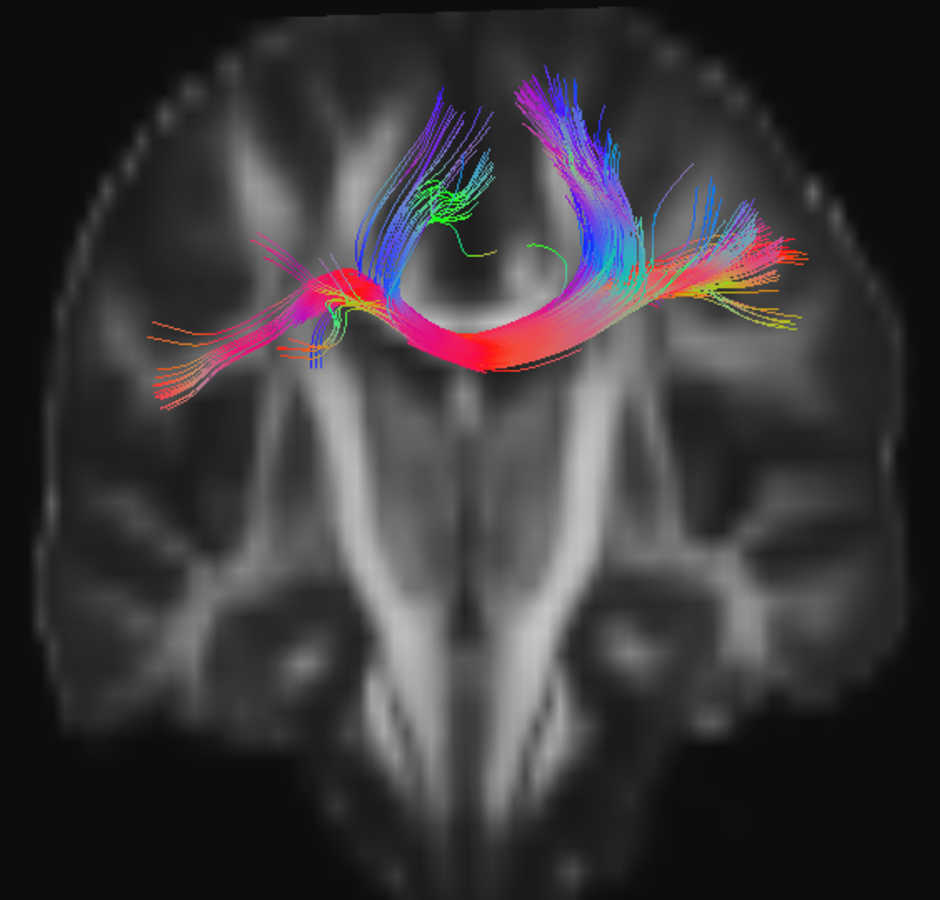
\includegraphics[width=0.4\textwidth]{Images/tracto_corps_calleux.pdf}
    \caption{\label{fig:tracto_corps_calleux}Fibres du corps calleux représentées sur une coupe coronale.}
\end{figure}

Le \tabref{tab:description} récapitule les différentes propriétés des molécules d'eau dans les trois tissus qui composent le cerveau.
\begin{table}[ht]
    \centering
    \begin{tabular}{D{5cm}||D{3cm}|D{3cm}}
	\textbf{Tisus} & \textbf{FA} & \textbf{DM} \tabularnewline
	\hline
	Liquide céphalorachidien & faible & élévée \tabularnewline
	Substance grise & faible & faible \tabularnewline
	Substance blanche & élevée & $\ast$ \tabularnewline
	\hline
    \end{tabular}
    \caption{\label{tab:description}Récapitulatif des propriétés de la diffusion de molécules d'eau 
    dans le liquide céphalorachidien, la substance grise et la substance blanche.}
\end{table}


\section{Pathologies neurodégénératives}
Nous retenons principalement du paragraphe précédent que, dans la substance blanche, la diffusion des molécules d'eau informe sur l'agencement des axones.
De manière intuitive, il est facile d'imaginer que si nous comparons deux régions spécifiques de ce tissu, 
appartenant à deux individus distincts et ayant un agencement différent,
il est possible de faire ressortir cette disparité.

Dans cette section, nous allons faire le lien entre l'utilisation de l'Imagerie du Tenseur de Diffusion
et les pathologies dégénératives du système nerveux central chez l'homme étudiées au cours de la thèse.
Une description succincte des atteintes de ces pathologies et des troubles qu'elles engendrent suivent.

Elles provoquent une mort lente et progressive des neurones, un vieillissement du cerveau,
ainsi qu'un problème de transmission de l'influx nerveux.
Notamment, et c'est qui nous intéressent plus particulièrement, elles s'attaquent à la gaine de myéline des axones, provoquant une \og démyélinisation \fg (\figref{fig:neurone}).
En reprenant l'analogie avec les câbles électriques, nous pouvons illustrer la démyélinisation par des câbles mis à nu.
Cela a pour conséquence de perturber l'influx nerveux entre les neurones.

La diffusion le long d'axones sains diffère de celle le long d'axones endommagés.
Par conséquent, la diffusion est un biomarqueur important pour mettre en évidence les régions du cerveau affectées par les pathologies neurodégénératives.



% De plus, nous nous sommes concentrés sur des pathologies de type démenciel. 
% explication de démence
% 
% maladie encore mal connues donc sujet d'étude important\\

\begin{figure}[ht]
    \centering
    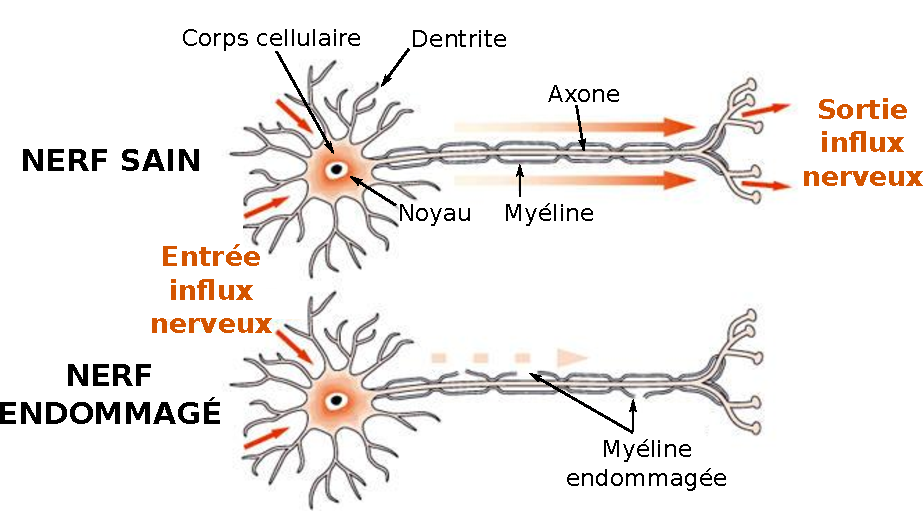
\includegraphics[width=1\textwidth]{Images/neurone.pdf}
    \caption{\label{fig:neurone}Illustration d'une démyélinisation}
\end{figure}

% divers troubles peuvent apparaître : 
% troubles moteurs,
% troubles visuels,
% troubles cognitifs
% 
% Les troubles de certaines maladies au stade prodromal se ressemble énormément et les pathologies peuvent donc être confondues.\\
% Cette erreur peut engendrer une prise de médicaments non adaptée pour le patient et une perte de temps importante pour le praticien


\section{Limites du modèle d'ordre 2}
limites du modèle d'ordre 2 pour représenter les croisements de fibres


\begin{figure}[ht]
    \centering
    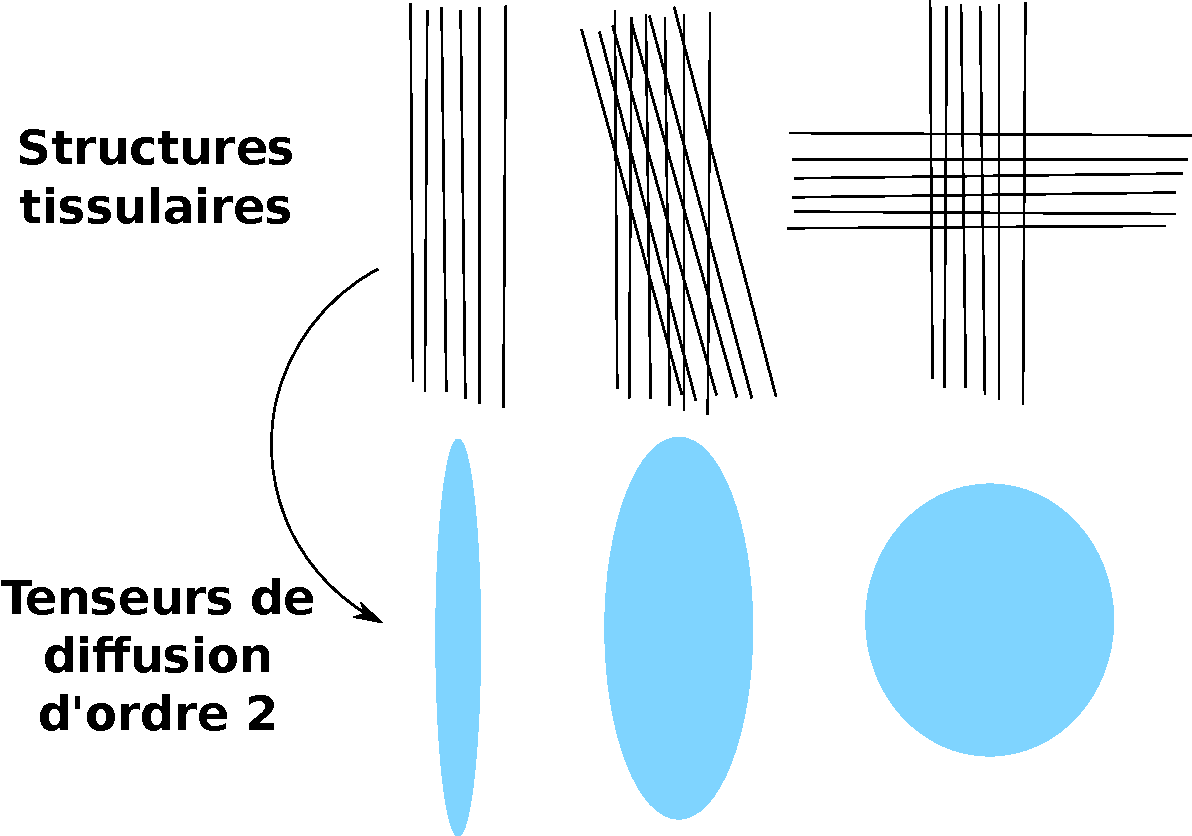
\includegraphics[width=0.5\textwidth]{Images/limite_tenseur.pdf}
    \caption{\label{fig:limite_tenseur}}
\end{figure}